\documentclass[tikz]{standalone}% 'crop' is the default for v1.0, before it was 'preview'
%\usetikzlibrary{...}% tikz package already loaded by 'tikz' option
\begin{document}
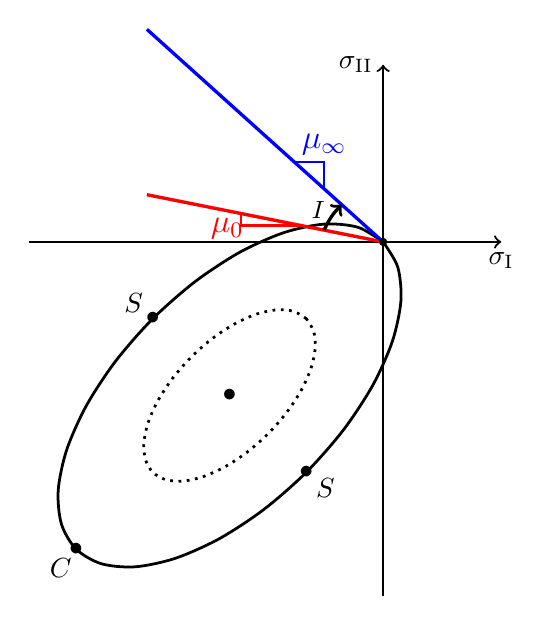
\begin{tikzpicture}[scale = 1.5]

    \draw [line width=1pt] [domain=0:2*pi,scale=0.65] plot[smooth] ({-2+2*cos(\x r)-sin(\x r)},{-2+sin(\x r)+2*cos(\x r)});
    \draw [line width=1pt,dotted] [domain=0:2*pi,scale=0.65] plot[smooth] ({-2+cos(\x r)-1/2*sin(\x r)},{-2+1/2*sin(\x r)+cos(\x r)});
    \draw [scale=0.65] (-2,-2) node {$\bullet$};
    \draw [scale=0.65] (-4,-4) node {$\bullet$};
    \draw [scale=0.65] (-3,-1) node {$\bullet$};
    \draw [scale=0.65] (-1,-3) node {$\bullet$};
    \draw [scale=0.65] (-4.2,-4) node[below] {$C$};
    \draw [scale=0.65] (-3,-0.8) node[left] {$S$};
    \draw [scale=0.65] (-1,-3.2) node[right] {$S$};
    % \draw [scale=0.65] (-0.1,-2) -- (0.1,-2) node[right]  {$-\frac{P}{2}$};
    % \draw [scale=0.65] (-2,-0.1) -- (-2,0.1) ;
    
    % \node at (-1.3, -0.3) {$-\frac{P}{2}$};

    \def \m {0.2}
    \def \n {0.9}

    \draw[thick, ->] (0, -3) -- (0, 1.5) node[left] {$\sigma_\mathrm{II}$};
    \draw[thick, ->] (-3, 0) -- (1, 0) node[below] {$\sigma_\mathrm{I}$};


    \draw[ red, very thick] (0, 0) -- (-2, 2*\m);
    \draw[ blue, very thick] (0, 0) -- (-2, 2*\n);

    % \draw[ red] (0, 0) -- (1, 2*\m) ;
    % \draw[ blue] (0, 0) -- (1, 2*\n);

    \draw[blue, thick] (-0.5,0.5*\n) |-(-0.75,\n*0.75) ;
    \node[blue] at (-0.5,0.82) {\large $\mu_\infty$};

    \draw[red, thick] (-1.2,1.2*\m) |-(-0.7,\m*0.7) ;
    \node[red] at (-1.32,0.11) {\large $\mu_0$};

    \draw[->, black, very thick] (-0.5, 0.5*\m) to [bend left=10] (-0.35,\n*0.35) ;
    \node[black] at (-0.55,0.27) {\small $I$};
    \draw [fill] (0,0) circle (0.03cm);



\end{tikzpicture}
\end{document}